%!TEX root = /Users/louis/Documents/PhD/Deliverables/Thesis/thesis.tex

\section[An Analysis of Languages used for Model Migration][An Analysis of Model Migration Languages]{An Analysis of Languages used for Model Migration}
\label{sec:analyis_of_languages_used_for_migration}
In contrast to the previous section, this section focuses on \emph{developer-driven} co-evolution, in which migration is specified as a program that metamodel users execute to migrate their models. Section~\ref{subsec:co-evolution_categorisation} discussed existing approaches to model migration, highlighting variation in the languages used for specifying migration strategies. In this section, the results of comparing migration strategy languages are described, using a new example of metamodel evolution (Section~\ref{subsec:co-evo_example}). From the comparison, requirements for a domain-specific language for specifying and executing model migration strategies are derived (Section~\ref{subsec:analysis}). The sequel describes an implementation of a model migration language based on the analysis presented here. The work described in this section has been published in \cite{rose10flock}.

\subsection{Co-Evolution Example}
\label{subsec:co-evo_example}
This section uses the Petri net metamodel evolution to compare model migration languages. The example is often used in co-evolution literature, for example \cite{cicchetti08automating,garces09managing,wachsmuth07metamodel}.

In Figure~\ref{fig:original_mm}, a Petri \texttt{Net} is defined to comprise \texttt{Pl\-a\-ce}s and \texttt{Tr\-an\-si\-ti\-on}s. A \texttt{Pl\-a\-ce} has any number of \texttt{src} or \texttt{dst} \texttt{Tr\-an\-si\-ti\-on}s. Similarly, a \texttt{Tr\-an\-si\-ti\-on} has at least one \texttt{src} and \texttt{dst} \texttt{Pl\-a\-ce}. The metamodel is to be evolved to support weighted connections between \texttt{Pl\-a\-ce}s and \texttt{Tr\-an\-si\-ti\-on}s and between \texttt{Tr\-an\-si\-ti\-on}s and \texttt{Pl\-a\-ce}s, as shown in Figure~\ref{fig:evolved_mm}. \texttt{Pl\-a\-ce}s are connected to \texttt{Tr\-an\-si\-ti\-on}s via instances of \texttt{PTArc}. Likewise, \texttt{Tr\-an\-si\-ti\-on}s are connected to \texttt{Pl\-a\-ce}s via \texttt{TPArc}. Both \texttt{PTArc} and \texttt{TPArc} inherit from \texttt{Arc}, and therefore can be used to specify a \texttt{we\-ig\-ht}.

\begin{figure}[htb]
	\centering
	\subfigure[Original metamodel.]
	{
	    \label{fig:original_mm}
	    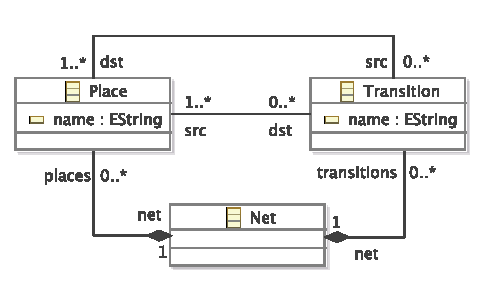
\includegraphics[scale=0.72]{5.Implementation/images/petri_nets_before.pdf}
	}
	\subfigure[Evolved metamodel.]
	{
	    \label{fig:evolved_mm}
	    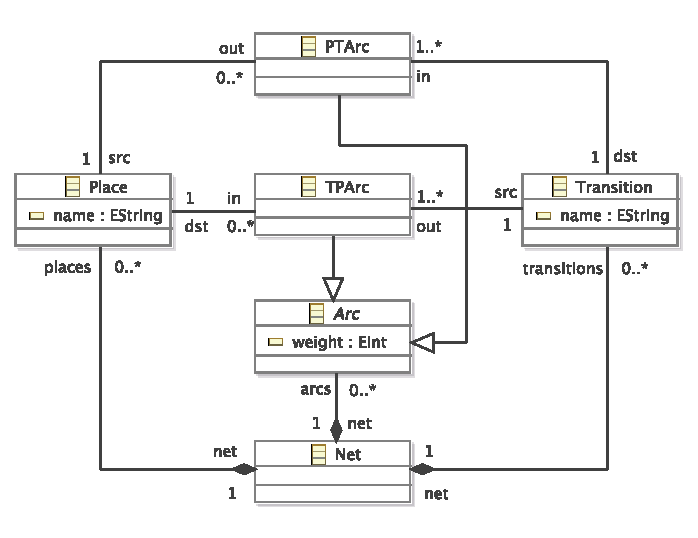
\includegraphics[scale=0.72]{5.Implementation/images/petri_nets_after.pdf}
	}
	\caption[Petri nets metamodel evolution]{Petri nets metamodel evolution. Taken from \cite{rose10flock}.}
\label{fig:petri_nets_mms}
\end{figure}

Models that conform to the original metamodel might not conform to the evolved metamodel. The following strategy can be used to migrate models:

\begin{enumerate}
	\item For every instance, t, of \texttt{Transition}: 
	\subitem For every \texttt{Place}, s, referenced by the \texttt{src} feature of t: 
	\subsubitem Create a new instance, arc, of \texttt{PTArc}. 
	\subsubitem Set s as the \texttt{src} of arc. 
	\subsubitem Set t as the \texttt{dst} of arc. 
	\subsubitem Add arc to the \texttt{arcs} reference of the \texttt{Net} referenced by t.
	
	\subitem For every \texttt{Place}, d, referenced by the \texttt{dst} feature of t: 
	\subsubitem Create a new instance, arc, of \texttt{TPArc}. 
	\subsubitem Set t as the \texttt{src} of arc. 
	\subsubitem Set d as the \texttt{dst} of arc. 
	\subsubitem Add arc to the \texttt{arcs} reference of the \texttt{Net} referenced by t.
	
	\item And nothing else changes.
\end{enumerate}

\subsection{Languages Currently Used for Model Migration}
\label{subsec:existing_migration_languages}
Using the above example, the languages used by existing approaches for specifying and executing model migration strategies are now compared. From this comparison, the strengths and weakness of each language are highlighted and requirements for a model migration language are synthesised in the sequel.

\subsubsection{Manual Specification with M2M Transformation}
\label{subsubsec:m2m}
Model migration can be specified using M2M transformation. For example, the Petri net migration has been specified in the Atlas Transformation Language (ATL) \cite{jouault05transforming}. This is reproduced in Listing~\ref{lst:atl}. Rules for migrating \texttt{Places} and \texttt{TPArcs} have been omitted for brevity, but are similar to the \texttt{Nets} and \texttt{PTArcs} rules.

Model transformation in ATL is specified using \texttt{rule}s, which transform source model elements (specified using the \texttt{fr\-om} keyword) to target model elements (specified using \texttt{to} keyword). For example, the \texttt{Nets} rule on line 1 of Listing~\ref{lst:atl} transforms an instance of \texttt{Net} from the original (source) model to an instance of \texttt{Net} in the evolved (target) model. The source model element (the variable \texttt{o} in the \texttt{Net} rule) is used to populate the target model element (the variable \texttt{m}). ATL allows rules to be specified as \emph{lazy} (not scheduled automatically and applied only when called by other rules).

\begin{lstlisting}[float=tbp, caption={[Fragment of the Petri nets model migration in ATL]Fragment of the Petri nets model migration in ATL, taken from \cite{rose10flock}}, label=lst:atl, language=ATL]
rule Nets {
	from o : Before!Net
	to m : After!Net ( places <- o.places, transitions <- o.transitions )
}

rule Transitions {
	from o : Before!Transition
	to m : After!Transition (
			name <- o.name,
			"in" <- o.src->collect(p | thisModule.PTArcs(p,o)),
			out  <- o.dst->collect(p | thisModule.TPArcs(o,p))
		)
}

unique lazy rule PTArcs {
	from place : Before!Place, destination : Before!Transition
	to ptarcs : After!PTArc (
			src <- place, dst <- destination, net <- destination.net
		)
}
\end{lstlisting}

The \texttt{Transitions} rule in Listing~\ref{lst:atl} codifies in ATL the migration strategy described previously. The rule is executed for each \texttt{Transition} in the original model, \texttt{o}, and constructs a \texttt{PTArc} (\texttt{TPArc}) for each reference to a \texttt{Place} in \texttt{o.src} (\texttt{o.dst}). Lazy rules must be used to produce the arcs to prevent circular dependencies with the \texttt{Transitions} and \texttt{Places} rules. Here, ATL, a typical rule-based transformation language, is considered and model migration would be similar in QVT. With Kermeta, migration would be specified in an imperative style using statements for copying \texttt{Net}s, \texttt{Place}s and \texttt{Transition}s, and for creating \texttt{PTArc}s and \texttt{TPArc}s.

In model transformation, \cite{czarnecki06survey} identifies two common categories of relationship between source and target model, \emph{new-target} and \emph{existing-target}. In the former, the target model is constructed afresh by the execution of the transformation, while in the latter, the target model contains the same data as the source model before the transformation is executed. M2M transformation languages typically support new-target transformations. Some M2M transformation languages also support existing-target transformations, but typically require the source and target metamodel to be identical.

In model migration, source and target metamodels differ, and therefore existing-target transformations cannot be used to specify model migration strategies. Consequently, model migration strategies are specified with new-target model-to-model transformation languages, and often contain sections for copying from original to migrated model those model elements that have not been affected by metamodel evolution. For the Petri nets example, the \texttt{Nets} rule (in Listing~\ref{lst:atl}) and the \texttt{Places} rule (not shown) exist only for this reason.


\subsubsection{Manual Specification with a Metamodel Mapping}
\label{subsubsec:ecore2ecore}
Model migration can be undertaken using the model loading mechanisms of EMF \cite{hussey06advanced}, with a tool that is termed \emph{Ecore2Ecore} here. EMF binds models to a specific metamodel, and hence cannot be used to load models that have been affected by metamodel evolution (Section~\ref{subsec:modelling_framework_characteristics}). Therefore, Ecore2Ecore requires the metamodel developer to provide a mapping between the metamodelling language of EMF (Ecore) and the concrete syntax used to persist models (XMI). Mappings are specified using Ecore2Ecore, which can suggest relationships between source and target metamodel elements by comparing names and types. Figure~\ref{fig:petri_nets_ecore2ecore} shows mappings between the original and evolved Petri nets metamodels.

\begin{figure}[htb]
	\centering
		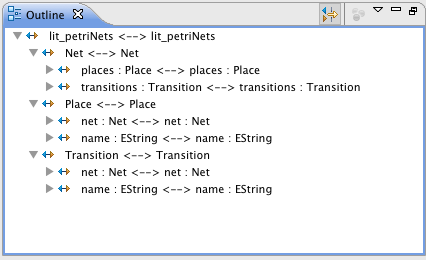
\includegraphics[scale=0.75]{5.Implementation/images/petri_nets_ecore2ecore.png}
	\caption[Mappings between the original and evolved Petri nets metamodels]{Mappings between the original and evolved Petri nets metamodels, constructed with the tool described in \cite{hussey06advanced}}
	\label{fig:petri_nets_ecore2ecore}
\end{figure}


The mappings are used by the EMF XMI parser to determine the metamodel types to which pieces of the XMI will be bound. When a type or feature is not bound, the user must specify a custom migration strategy in Java. For the Petri nets metamodel, the \texttt{src} and \texttt{dst} features of \texttt{Place} and \texttt{Transition} are not bound, because migration is more complicated than a one-to-one mapping.

\begin{lstlisting}[float=tbp, caption=Java method for deserialising a reference., label=lst:java, language=Java]
private Collection<Place> toCollectionOfPlaces
(String value, Resource resource) {

  final String[] uriFragments    = value.split(" ");
  final Collection<Place> places = new LinkedList<Place>();
 
  for (String uriFragment : uriFragments) {
		final EObject eObject = resource.getEObject(uriFragment);
		final EClass place    = PetriNetsPackage.eINSTANCE.getPlace();

    if (eObject == null || !place.isInstance(eObject))
      // throw an exception
						
		places.add((Place)eObject);
  }
 
  return places;
}
\end{lstlisting}

In Ecore2Ecore, model migration is specified on the XMI representation of the model and requires some knowledge of the XMI standard. For example, in XMI, references to other model elements are serialised as a space delimited collection of URI fragments \cite{steinberg09emf}. Listing~\ref{lst:java} shows a fragment of the code used to migrate Petri net models with Ecore2Ecore. The method shown converts a \texttt{String} containing URI fragments to a \texttt{Collection} of \texttt{Place}s. The method is used to access the \texttt{src} and \texttt{dst} features of \texttt{Tr\-an\-si\-ti\-on}, which no longer exist in the evolved metamodel and hence are not loaded automatically by EMF. To specify the migration strategy for the Petri nets example, the metamodel developer must know the way in which the \texttt{src} and \texttt{dst} features are represented in XMI. The complete listing (presented in Section~\ref{sec:ecore2ecore_listings}) exceeds 150 lines of code.

\subsubsection{Operator-based Co-evolution with COPE}
\label{subsubsec:cope}

Operator-based approaches to identifying and managing co-evolution, such as COPE \cite{herrmannsdoerfer09cope}, provide a library of \emph{co-evolutionary operators}. Each co-evolutionary operator specifies both a metamodel evolution and a corresponding model migration strategy. For example, the ``Make Reference Containment'' operator from COPE \cite{herrmannsdoerfer09cope} evolves the metamodel such that a non-containment reference becomes a containment reference and migrates models such that the values of the evolved reference are replaced by copies. By composing co-evolutionary operators, metamodel evolution can be performed and a migration strategy can be generated without writing any code.

Clearly, the development of an operator-based approach must start by identifying operators, which can be challenging. Operators capture both metamodel evolution and model migration semantics, and as such, a complete library of operators is difficult to imagine \cite{lerner00model}. Instead, operator-based approaches seek to capture the most commonly occurring co-evolutionary operators, which are typically identified by examining existing examples of evolution \cite{herrmannsdoerfer08automatability}. Hence, the breadth of consultation when identifying operators will affect the efficacy of an operator-based approach, because evolutionary changes that occur frequently in one project might never occur in other projects, or vice-versa.

To perform metamodel evolution using an operator-based approach, the library of co-evolutionary operators must be integrated with tools for editing metamodels. COPE provides integration with the EMF tree-based metamodel editor. Operators may be applied to an EMF metamodel, and COPE tracks their application. Once metamodel evolution is complete, a migration strategy can be generated automatically from the record of changes maintained by COPEs. The migration strategy is distributed along with the updated metamodel, and metamodel users choose when to execute the migration strategy on their models.

\begin{lstlisting}[float=tbp, caption=Petri nets model migration in COPE, label=lst:cope, language=COPE]
for (transition in petrinets.Transition.allInstances) {
  for (source in transition.unset('src')) {
    def arc = petrinets.PTArc.newInstance()
    arc.src = source
    arc.dst = transition
    arc.net = transition.net
  }
  
  for (destination in transition.unset('dst')) {
    def arc = petrinets.TPArc.newInstance() 
    arc.src = transition
    arc.dst = destination
    arc.net = transition.net
  }
}

for (place in petrinets.Place.allInstances) {
  place.unset('src')
  place.unset('dst')
}
\end{lstlisting}

To be effective, operator-based approaches must provide a rich yet navigable library of co-evolutionary operators (Section~\ref{subsec:co-evolution_categorisation}). COPE allows model migration strategies to be specified manually when no co-evolutionary operator is appropriate. COPE employs a fundamentally different approach to M2M transformation and Ecore2Ecore, using an existing-target transformation. As discussed above, existing-target transformations cannot be used for specifying model migration strategies as the source (original) and target (evolved) metamodels differ. However, models can be structured independently of their metamodel using a metamodel-independent syntax (such as the one introduced in Section~\ref{sec:mmi_syntax}).

Listing~\ref{lst:cope} shows the COPE model migration strategy for the Petri net example given above\footnote{In Listing~\ref{lst:cope}, some of the concrete syntax has been changed in the interest of readability.}. Most notably, slots for features that no longer exist must be explicitly \texttt{unset}. In Listing~\ref{lst:cope}, slots are \texttt{unset} on four occasions (on lines 2, 9, 18 and 19), once for each feature that is in the original metamodel but not in the evolved metamodel. These features are: \texttt{src} and \texttt{dst} of \texttt{Transition} and of \texttt{Place}. Failing to unset slots that do not conform to the evolved metamodel causes migration to fail with an error.

\subsection{Requirements Identification}
\label{subsec:analysis}
Requirements for a domain-specific for model migration were identified from the review of existing languages (Section~\ref{subsec:existing_migration_languages}). The derivation of the requirements is now summarised, by considering two orthogonal concerns: the source-target relationship of the language used for specifying migration strategies and the way in which models are represented during migration. %and the structures provided by the language for specifying and re-using migration strategies.


\subsubsection{Source-Target Relationship Requirements}
When migration is specified as a new-target transformation, as in ATL (Listing~\ref{lst:atl}), model elements that have not been affected by metamodel evolution must be explicitly copied from the original to the migrated model. When migration is specified as an existing-target transformation, as in COPE (Listing~\ref{lst:cope}), model elements and values that no longer conform to the target metamodel must be explicitly removed from the migrated model. Ecore2Ecore does not require explicit copying or unsetting code; instead, the relationship between original and evolved metamodel elements is captured in a mapping model specified by the metamodel developer. The mapping model can be derived automatically and customised by the metamodel developer. To explore the appropriateness for model migration of an alternative to new- and existing-target transformations, the following requirement was derived:

\emph{The migration language must \textbf{automatically} copy every model element that conforms to the evolved metamodel from original to migrated model, and must automatically not copy any model element that does not conform to the evolved metamodel from original to migrated model.}


\subsubsection{Model Representation Requirements}
With Ecore2Ecore, migration is achieved by manipulating XMI. Consequently, the metamodel developer must be familiar with XMI and must perform tasks such as dereferencing URI fragments (Listing~\ref{lst:java}) and type conversion. Transformation languages abstract over the underlying storage representation of models (such as XMI) by using a modelling framework to load, store and access models.

\emph{The migration language must not expose the underlying representation of models.}

\vspace{5mm}

To apply co-evolution operators, COPE requires the metamodel developer to use a specialised metamodel editor. The editor can manipulate only metamodels defined with EMF. Similarly, the mapping tool used in the Ecore2Ecore approach can be used only with metamodels defined with EMF. Although EMF is arguably very widely-used, other modelling frameworks exist. Adapting to interoperate with new systems is recognised as a common reason for software evolution \cite{sjoberg93quantifying}, and migration between modelling frameworks is as a possible use case for a model migration language. In particular, there is demand for migrating between UML 1 (e.g. \cite{uml14}) and UML 2 (e.g. \cite{uml22}) models\footnote{Forum discussion with Tom Morris, lead developer of the ArgoUML tool, \url{http://www.planet-research20.org/ttc2010/index.php?option=com_community&view=groups&task=viewdiscussion&groupid=4&topicid=20&Itemid=150} (registration required).}, which are typically managed with different modelling frameworks. Decoupling model management operations from the model representation facilitates interoperability with many modelling technologies, as demonstrated by Epsilon (Section~\ref{subsec:epsilon}). Therefore, to facilitate interoperability with modelling frameworks other than EMF, the following requirement was derived:

\emph{The migration language must be loosely coupled with modelling frameworks and must not assume that models and metamodels will be represented in EMF.}